\documentclass{article}
\usepackage{float}
\usepackage{graphicx}
\usepackage{indentfirst}
\usepackage[a4paper, total={6in, 8in}]{geometry}
\usepackage{hyperref}
\usepackage{fancyhdr}
\usepackage{xepersian}
\settextfont{B Nazanin}
\setlatintextfont{Times New Roman}

\begin{document}


%title page%
\begin{titlepage}
	\begin{center}
		\textbf{ \Huge{به نام خدا}}
	
		\vspace{0.2cm}
		
		
\includegraphics[width=0.4\textwidth]{sharif.png}\\
		\vspace{0.2cm}
		\textbf{ \Huge{آزمایش شماره ۱}}\\
		\vspace{0.25cm}
		\textbf{ \Large{آز معماری - دکتر سربازی آزاد}}
		\vspace{0.2cm}
		
		
		\large \textbf{دانشکده مهندسی کامپیوتر}\\\vspace{0.1cm}
		\large   دانشگاه صنعتی شریف\\\vspace{0.2cm}
		\large   ﻧﯿﻢ‌سال اول ۰۰-۰۱ \\\vspace{0.10cm}
		\large{گروه :}\\
		\large{\href{mailto:a.h.hadian@gmail.com}{امیرحسین هادیان - ۹۷۱۰۲۶۰۹}}\\
		\large{\href{mailto:mofayezi.m@gmail.com}{محمدرضا مفیضی - ۹۸۱۰۶۰۵۹}}\\
		\large{\href{mailto:a.hatam008@gmail.com}{علی حاتمی تاجیک - ۹۸۱۰۱۳۸۵}}\\
	\end{center}
\end{titlepage}
%title page%

\newpage

%pages header
\pagestyle{fancy}
\fancyhf{}
\fancyfoot{}
\setlength{\headheight}{59pt}
\cfoot{\thepage}
\lhead{آزمایش شماره ۱}
\rhead{
\includegraphics[width=0.1\textwidth]{sharif.png}\\
		دانشکده مهندسی کامپیوتر
}
\chead{آز معماری}
%pages header

\section{مقدمه}
در این سند گزارشی بر روند طراحی، پیاده‌سازی و تست یک مدار جمع کننده \lr{BCD} سه رقمی آورده ‌شده است. برای شبیه‌سازی این طراحی از نرم‌افزار \lr{Proteus} استفاده شده است. فایل پروژه از این لینک قابل مشاهده است.

\section{هدف}
هدف از انجام این آزمایش طراحی و ساخت یک جمع‌کننده ده‌دهی سه‌رقمی است. این جمع کننده ترکیبی خواهد بود و با تغییر ورودی‌ها تغییرات مستقیما در خروجی نمایان خواهند شد.

\section{طراحی}
طراحی این مدار به صورت سلسله مراتبی و \lr{Top-Down} صورت گرفته است. به همین‌ صورت نیز توضیح داده خواهد شد. در بالاترین لایه جمع‌کننده ده‌دهی سه بیتی ما به همراه کلید‌های ورودی و نمایشگر‌های \lr{7-Segments} قرار دارند که ورودی‌ها و نتیجه خروجی‌ را به ما نمایش می‌دهند. برای متصل کردن هر عدد ده‌رقمی از یک خط باس چهاربیتی استفاده شده است. از این خط باس در ماژول‌های پایین‌تر نیز برای تمیزی و سادگی نمایش بهره‌ برده شده است.
به ورودی
$ C_{in} $
 جمع‌کننده مقدار ثابت صفر وارد می‌شود. همینطور در در نمایش سه پایه نمایشگر به زمین متصل شده‌اند چرا که همواره صفر خواهند بود و تنها پایه اول که به
$C_{out}$
  متصل است (بزرگترین عددی که ممکن است تولید شود عدد 1999 خواهد بود). بالاترین سطح طراحی در شکل \ref{fig:final} آمده است.

\begin{figure}
	\centering
	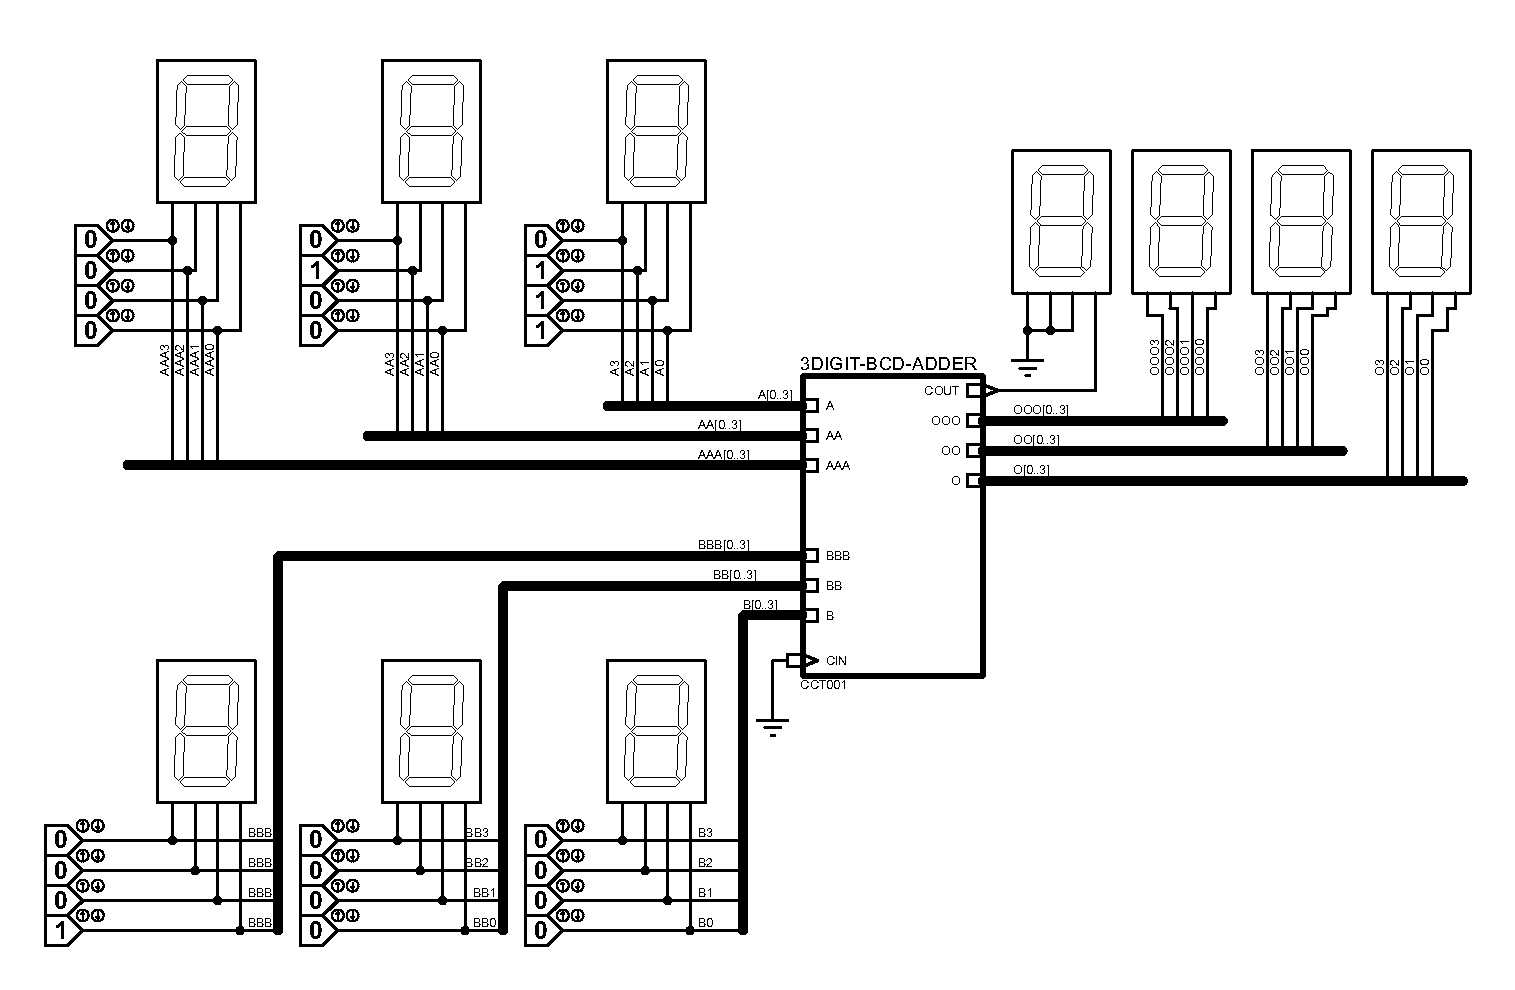
\includegraphics[scale=0.5]{./captures/final}
	\caption{مدار نهایی}
	\label{fig:final}
\end{figure}

\subsection{جمع‌کننده دهدهی سه رقمی}
این ماژول جمع کننده دارای ۶ ورودی باس چهار بیتی است که سه‌ تای آن مربوط به عدد دهدهی اول و سه تای آن مربوط به عدد دهدهی دوم است. درون این ماژول سه جمع‌کننده دهدهی یک بیتی وجود دارد که از هر کدام برای جمع کردن رقم‌های از یک مرتبه ارزش اعداد ورودی استفاده می‌شود. این بیت نقلی این جمع کننده‌ها به صورت آبشاری به جمع‌کننده مرتبه بالاتر انتقال می‌یابد. برای زیبایی و سادگی همان باس‌های ورودی به ورودی جمع کننده‌های یک رقمی وارد می‌شوند. رقم نقلی جمع کننده سوم به عنوان رقم نقلی کل به خروجی می‌فرستیم. خروجی‌های چهاربیتی هر جمع کننده را نیز به عنوان خروجی همان مرتبه و به صورت یک خط باس چهاربیتی به خروجی ‌می‌فرستیم. منطق طراحی این بخش، مانند جمع زدن عادی است که ما انسان‌ها انجام می‌دهیم. ارقام را از مربته کوچک به بزرگ جمع می‌زنیم و اگر رقم نقلی داشتیم آنرا در مرتبه بعدی جمع می‌زنیم. در شکل \ref{fig:3bcd} داخل جمع کننده دهدهی سه‌رقمی آمده است.

\begin{figure}
	\centering
	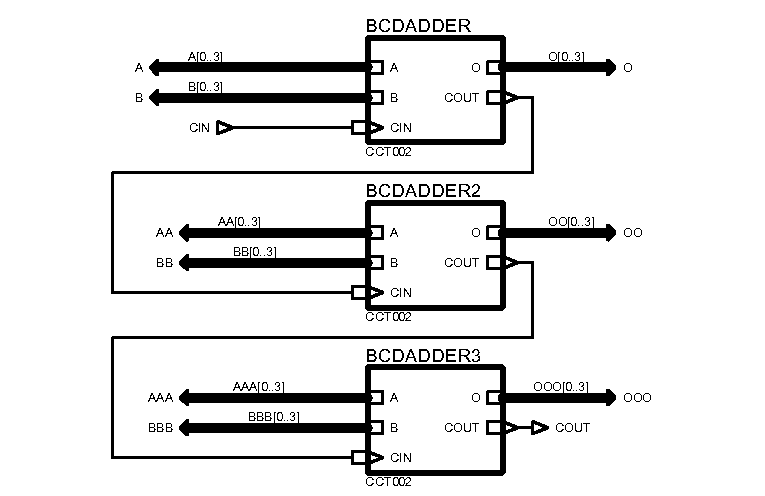
\includegraphics[scale=0.7]{./captures/3bcd}
	\caption{جمع‌کننده دهدهی سه‌رقمی}
	\label{fig:3bcd}
\end{figure}

\subsection{جمع‌کننده دهدهی برای یک رقم}
این جمع کننده دو خط باس چهاربیتی ورودی می‌گیرد و جمع آنها را به صورت یک خط باس چهاربیتی و یک بیت نقلی به خروجی می‌فرستد. روش کار آن به این صورت است که این دو عدد چهار بیتی به صورت بیتی جمع می‌زند. اگر جمع این دو عدد از عدد ۹ بیشتر باشد (در عدد ده، بیت دوم و چهارم یک می‌شود و در عدد‌های بزرگتر دو بیت آخر یک می‌شود و یا بیت نقلی جمع کننده چهاربیتی یک می‌شود) باید یک بیت نقلی به خارج بفرستیم و عدد حاصل جمع را هم با عدد ۶ جمع کنیم. برا این کار به این صورت عمل می‌کنیم که ابتدا اینکه بیت نقلی داریم یا نه را با توجه به چیز‌هایی که گذشت پیدا می‌کنیم. این بیت اگر نیاز به جمع زدن با عدد ۶ داشته باشیم یک است و در غیر این صورت برابر با ۰ خواهد بود. حال یک جمع‌کننده چهاربیتی دیگر میگذاریم و عدد چهاربیتی حاصل جمع را با عدد $0cc0$ جمع میزنیم که در آن $c$ بیت نقلیمان است. اگر بیت نقلی یک باشد این مقدار برابر با ۶ و در غیر این صورت برابر با صفر خواهد بود که نتیجه جمع همان نتیجه مطلوب ما خواهد بود. برای طراحی این ماژول از چند گیت پایه و دو جمع کننده چهاربیتی استفاده شده است که در ادامه توضیح داده‌ خواهد شد. جمع کننده دهدهی برای یک رقم در شکل \ref{fig:bcd} آمده است. در این ماژول باس ورودی از هم تفکیک شده است و به صورت بیت به بیت به جمع‌کننده چهاربیتی وارد شده است..

\begin{figure}
	\centering
	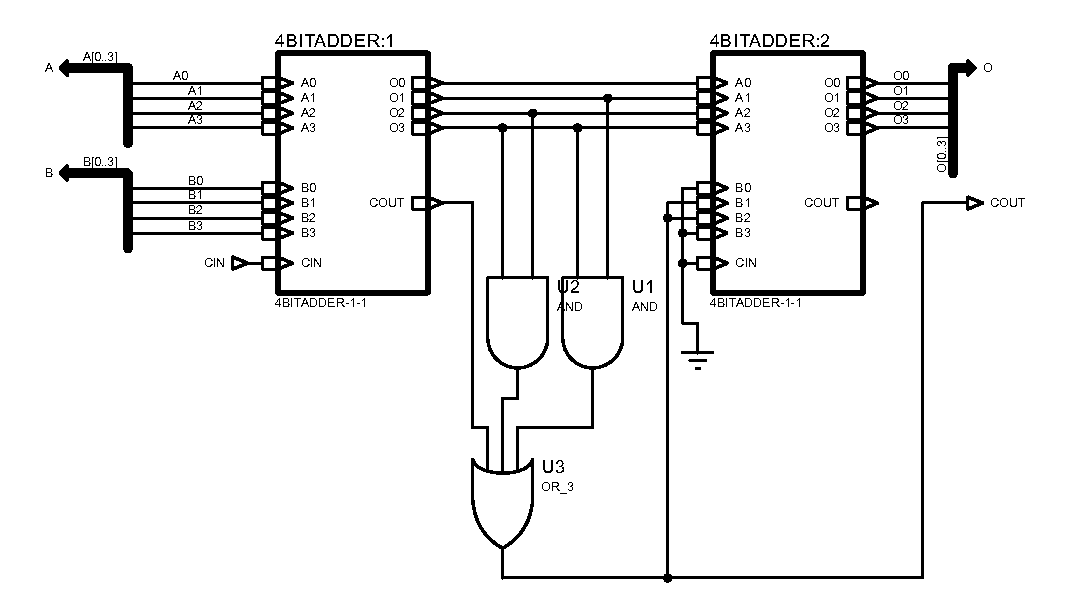
\includegraphics[scale=0.5]{./captures/bcd}
	\label{fig:bcd}
	\caption{جمع کننده دهدهی برای یک رقم}
\end{figure}

\subsection{جمع کننده چهاربیتی}
این جمع کننده دو عدد چهاربیتی را و یک بیت نقلی ورودی می‌گیرد و یک عدد چهار بیتی و یک بیت نقلی خروجی می‌دهد. ساخت آن به وسیله چهار تمام جمع‌کننده انجام می‌گیرد که به صورت آبشاری به یکدیگر متصل شده اند و بیت نقلی خروجی یکی بیت نقلی ورودی جمع کننده با مرتبه بیشتر خواهد بود. درون این جمع کننده چهاربیتی در شکل \ref{fig:4bit} آمده است. در این جمع کننده از تمام جمع کننده‌ها استفاده شده است که در ادامه ساختار آن توضیح داده خواهد شد.

\begin{figure}
	\centering
	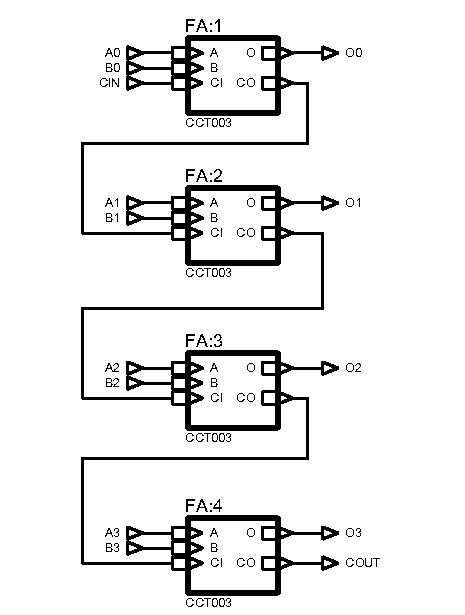
\includegraphics[scale=0.7]{./captures/4bit}
	\label{fig:4bit}
	\caption{جمع کننده کامل چهاربیتی}
\end{figure}

\subsection{تمام‌جمع‌کننده}
در شکل \ref{fig:fa} ساختار درونی تمام جمع‌کننده‌های استفاده شده در مدار آمده است. در داخل این تمام جمع کننده‌ از گیت‌های پایه بر اساس مطالب درس مدارهای منطقی استفاده شده است.

\begin{figure}
	\centering
	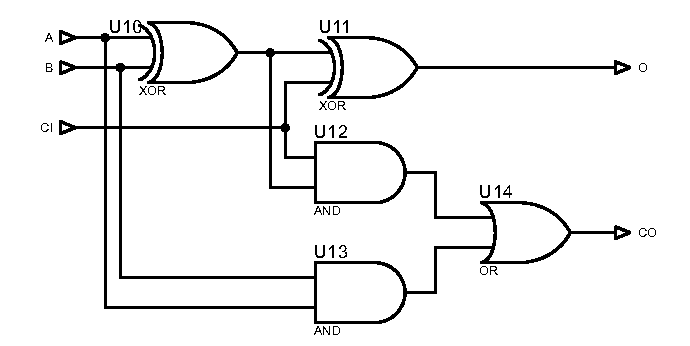
\includegraphics[scale=0.7]{./captures/fa}
	\caption{تمام جمع کننده}
	\label{fig:fa}
\end{figure}

\section{تست}
در این بخش چند دسته ورودی را بر روی مدار آزمایش شده‌اند و نتایج در اشکال پایین آمده اند. درستی نتایج در توضیحات هر عکس آورده شده است.  

\begin{figure}[H]
	\centering
	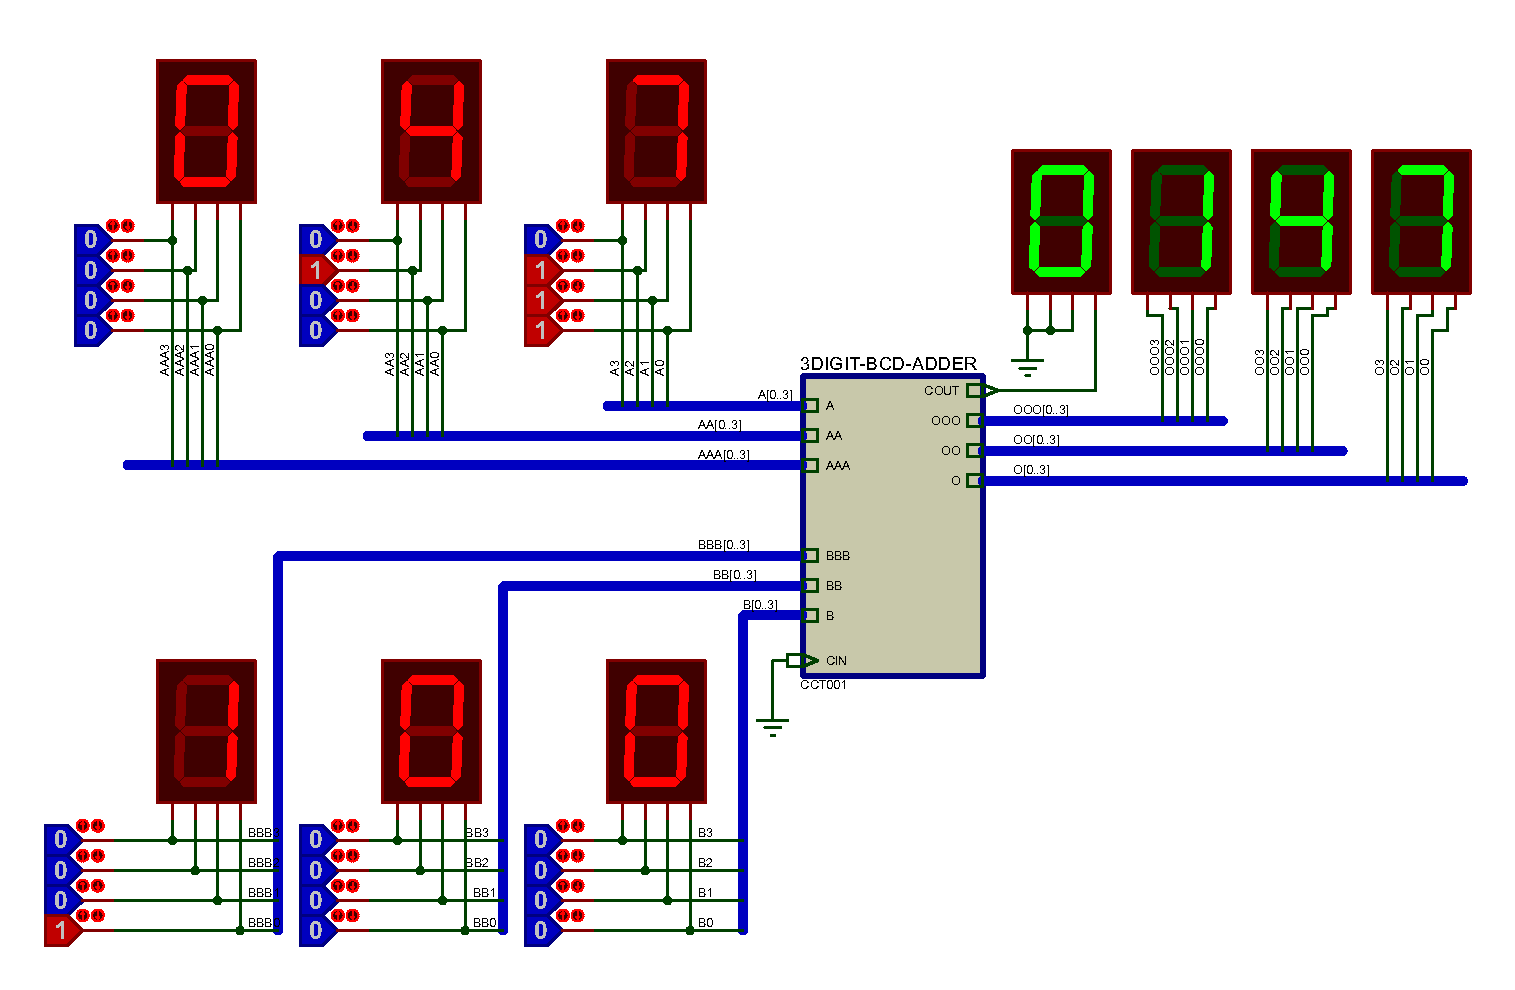
\includegraphics[scale=0.4]{./captures/test}
	\caption{$ 47 + 100 = 147 $}
\end{figure}

\begin{figure}[H]
	\centering
	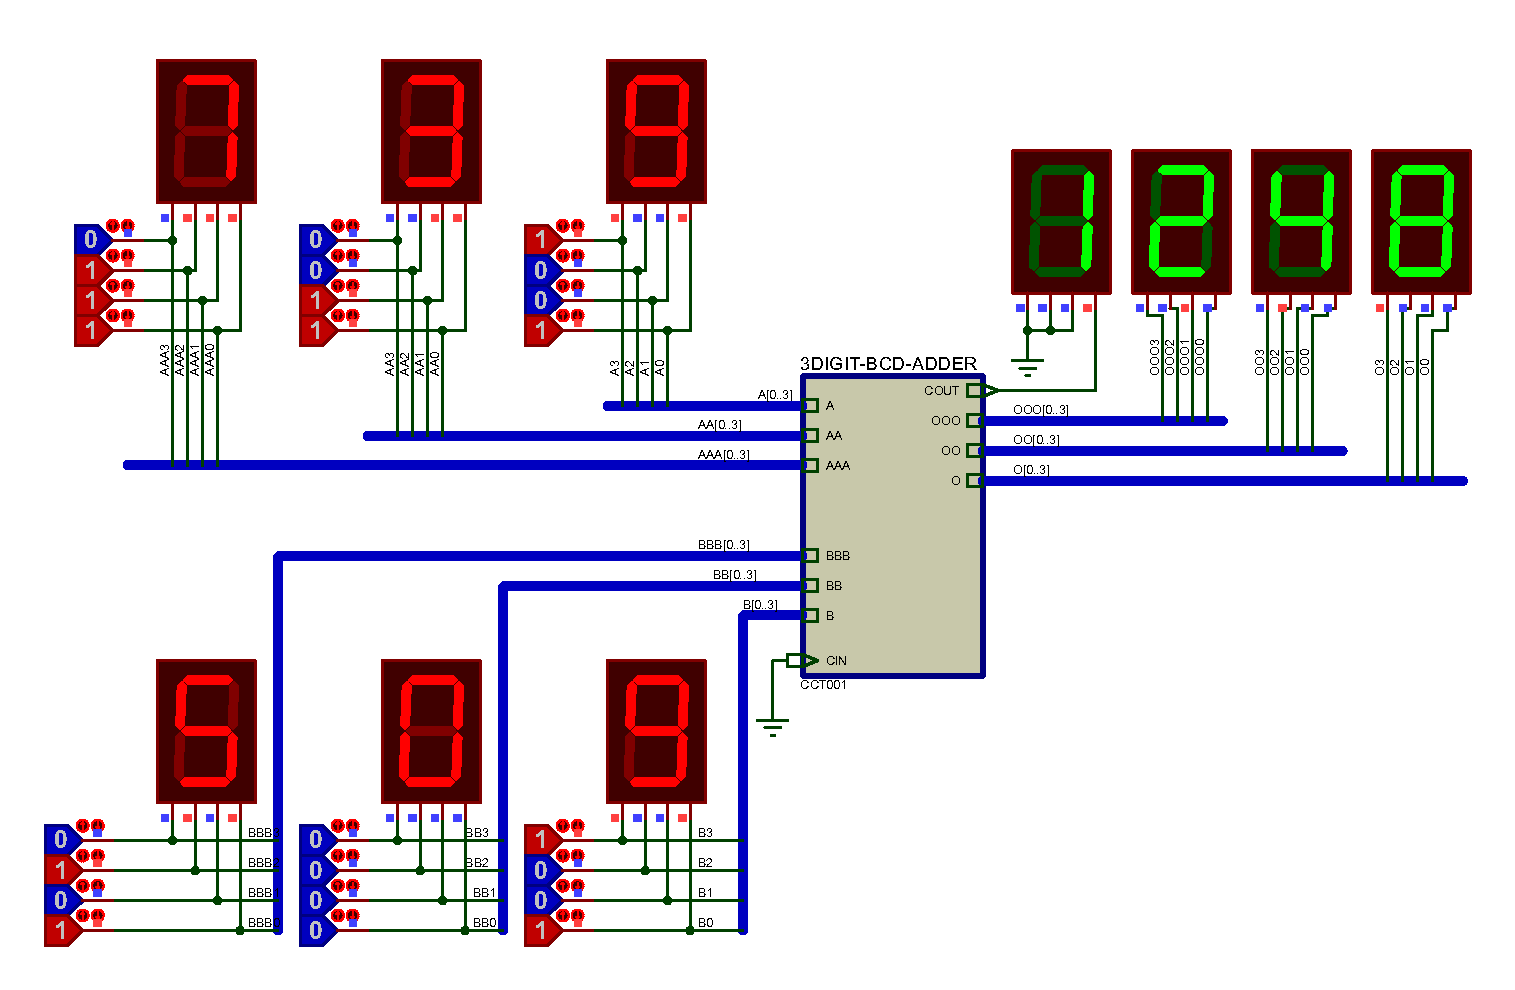
\includegraphics[scale=0.4]{./captures/test2}
	\caption{$ 739 + 509 = 1248 $}
\end{figure}


\begin{figure}[H]
	\centering
	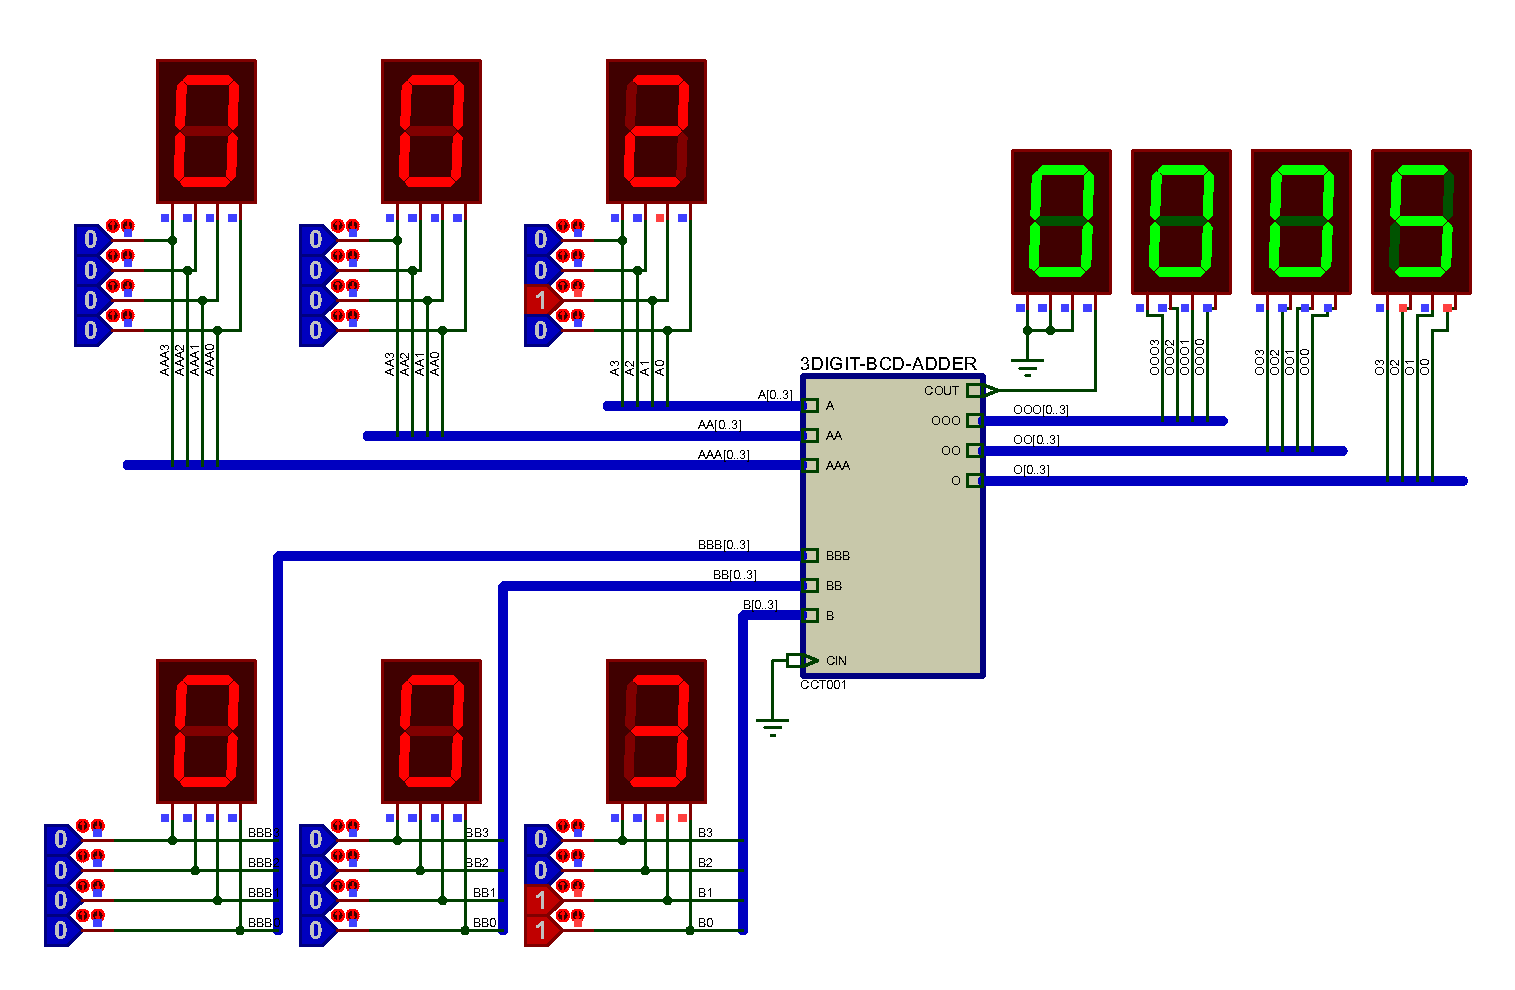
\includegraphics[scale=0.4]{./captures/test3}
	\caption{$ 2 + 3 = 5 $}
\end{figure}
\end{document}
